\documentclass[12pt]{article}\usepackage[]{graphicx}\usepackage[]{color}
%% maxwidth is the original width if it is less than linewidth
%% otherwise use linewidth (to make sure the graphics do not exceed the margin)
\makeatletter
\def\maxwidth{ %
  \ifdim\Gin@nat@width>\linewidth
    \linewidth
  \else
    \Gin@nat@width
  \fi
}
\makeatother

\definecolor{fgcolor}{rgb}{0, 0, 0}
\newcommand{\hlnum}[1]{\textcolor[rgb]{0,0,0}{#1}}%
\newcommand{\hlstr}[1]{\textcolor[rgb]{0,0,0}{#1}}%
\newcommand{\hlcom}[1]{\textcolor[rgb]{0.4,0.4,0.4}{\textit{#1}}}%
\newcommand{\hlopt}[1]{\textcolor[rgb]{0,0,0}{\textbf{#1}}}%
\newcommand{\hlstd}[1]{\textcolor[rgb]{0,0,0}{#1}}%
\newcommand{\hlkwa}[1]{\textcolor[rgb]{0,0,0}{\textbf{#1}}}%
\newcommand{\hlkwb}[1]{\textcolor[rgb]{0,0,0}{\textbf{#1}}}%
\newcommand{\hlkwc}[1]{\textcolor[rgb]{0,0,0}{\textbf{#1}}}%
\newcommand{\hlkwd}[1]{\textcolor[rgb]{0,0,0}{\textbf{#1}}}%
\let\hlipl\hlkwb

\usepackage{framed}
\makeatletter
\newenvironment{kframe}{%
 \def\at@end@of@kframe{}%
 \ifinner\ifhmode%
  \def\at@end@of@kframe{\end{minipage}}%
  \begin{minipage}{\columnwidth}%
 \fi\fi%
 \def\FrameCommand##1{\hskip\@totalleftmargin \hskip-\fboxsep
 \colorbox{shadecolor}{##1}\hskip-\fboxsep
     % There is no \\@totalrightmargin, so:
     \hskip-\linewidth \hskip-\@totalleftmargin \hskip\columnwidth}%
 \MakeFramed {\advance\hsize-\width
   \@totalleftmargin\z@ \linewidth\hsize
   \@setminipage}}%
 {\par\unskip\endMakeFramed%
 \at@end@of@kframe}
\makeatother

\definecolor{shadecolor}{rgb}{.97, .97, .97}
\definecolor{messagecolor}{rgb}{0, 0, 0}
\definecolor{warningcolor}{rgb}{1, 0, 1}
\definecolor{errorcolor}{rgb}{1, 0, 0}
\newenvironment{knitrout}{}{} % an empty environment to be redefined in TeX

\usepackage{alltt}

%%%%%%%%%%%%%%%%%%%%%%%%%%%%%%%%%%%%%%%% packages
\usepackage{float} % for better behaved floats
\usepackage{graphicx} % for pictures
\usepackage{fancyhdr} % for headers
\usepackage{verbatim} % displaying r code
%\usepackage{fancyvrb}
\usepackage{setspace} % vspace and hspace
%\usepackage{listings}
\usepackage{enumitem} % for [label=]
\usepackage{amsmath}  % math symbols and such
\usepackage{amssymb}
\usepackage{lastpage} % for page numerbering
\usepackage{color}
\usepackage{multirow}
% \usepackage[nottoc,numbib]{tocbibind} % Puts references in TOC
\usepackage{authblk}
\usepackage{framed}

%%%%%%%%%%%%%%%%%%%%%%%%%%%%%%%%%%%%%%%%%%%%%%%%%
%% Uncomment this line to hide the solutions
\usepackage[forcolorpaper,nopoints,nosolutions]{eqexam}

%% Uncomment this line to show the solutions
%\usepackage[forcolorpaper,nopoints,solutionsafter]{eqexam}
%%%%%%%%%%%%%%%%%%%%%%%%%%%%%%%%%%%%%%%%

\renameSolnAfterTo{\textcolor{blue}{\textit{Solution:}}}
\def\exrtnlabelformat{}
\def\exrtnlabelformatwp{}
\def\eq@sqslrtnlabel{}
  % \definecolor{shadecolor}{rgb}{1,0,0}


%%%%%%%%%%%%%%%%%%%%%%%%%%%%%%%%%%%%%%%% margins
\setlength{\textwidth}{6.5in}
\setlength{\textheight}{9in}
\setlength{\oddsidemargin}{0in}
\setlength{\evensidemargin}{0in}
\setlength{\topmargin}{-1.5cm}
\setlength{\parskip}{0pt} % No skip line before and after each par
\setlength{\parindent}{0pt} % No auto-indent
% \def\fs{\footnotesize}
%%%%%%%%%%%%%%%%%%%%%%%%%%%%%%%%%%%%%%%%%%%%%%%%%

%%%%%%%%%%%%%%%%%%%%%%%%%%%%%%%%%%%%%%%%%%%%%%%%%
%% tell knitr to use smaller font for code chunks
\ifdefined\knitrout
\renewenvironment{knitrout}{\begin{footnotesize}}{\end{footnotesize}}
\else
  \fi
\newcommand{\R}{{\sf R} }
\newcommand{\Rstud}{{\sf Rstudio} }

\newlength{\gap}
\setlength{\gap}{.2cm}
%%%%%%%%%%%%%%%%%%%%%%%%%%%%%%%%%%%%%%%%%%%%%%%%%

%%%%%%%%%%%%%%%%%%%%%%%%%%%%%%%%%%%%%%%% headers
\pagestyle{fancy} % headers
\lhead{STAT 217, Fall 2016}
\chead{Sep 9}
\rhead{Name:\hspace{4cm}}
\lfoot{}
\cfoot{}
\rfoot{}
\renewcommand{\headrulewidth}{2pt}
% \renewcommand{\footrulewidth}{1pt}
%%%%%%%%%%%%%%%%%%%%%%%%%%%%%%%%%%%%%%%%%%%%%%%%%
\IfFileExists{upquote.sty}{\usepackage{upquote}}{}
\begin{document}

\begin{center}
{\Large \bf Activity for 2 independent sample means:} \\
\end{center}

%%%%%%%%%%%%%%%%%%%%%%%%%%%%%%%%%%%%%%%% R code options

%%%%%%%%%%%%%%%%%%%%%%%%%%%%%%%%%%%%%%%%%%%%%%%%%

\subsection*{Description of {\tt snow1} dataset}

Karl Wetlaufer, Jordy Hendrikx, and Lucy Marshall wrote a paper for a journal on snow density (the full article is on D2L) and different areas of the West Fork of the Gallatin River Basin in southwest Montana. we will focus on two of the variables the team collected data on: snow depth ({\tt depth}) and forest cover ({\tt cover}). The snow depth was measured in mm and the areas either forested (a 10 was recorded) or unforested (a 0 was recorded). We want to investigate if this data suggest some association between forest cover and snow depth, on average. If there is an association, we would like to know by how much snow depth the areas might differ on average.

\subsection*{Explore the data}


\begin{knitrout}\footnotesize
\definecolor{shadecolor}{rgb}{1, 1, 1}\color{fgcolor}\begin{kframe}
\begin{alltt}
\hlcom{# TODO: load in the data and call it snow (on D2L it is snow1)}

\hlcom{# look at the summary statistics}
\hlkwd{require}\hlstd{(mosaic)}
\hlkwd{favstats}\hlstd{(depth} \hlopt{~} \hlstd{cover,} \hlkwc{data} \hlstd{= snow)}
\end{alltt}
\begin{verbatim}
##   cover min  Q1 median   Q3  max     mean       sd   n missing
## 1     0   0 152    940 1219 2540 793.5228 603.4008 614       0
## 2    10   0   0    432 1118 2743 646.8362 636.3934 403       0
\end{verbatim}
\end{kframe}
\end{knitrout}

\begin{knitrout}\footnotesize
\definecolor{shadecolor}{rgb}{1, 1, 1}\color{fgcolor}\begin{kframe}
\begin{alltt}
\hlcom{# look at the distributions}
\hlkwd{par}\hlstd{(}\hlkwc{mfrow} \hlstd{=} \hlkwd{c}\hlstd{(}\hlnum{1}\hlstd{,} \hlnum{2}\hlstd{))}
\hlkwd{boxplot}\hlstd{(depth} \hlopt{~} \hlstd{cover,} \hlkwc{data} \hlstd{= snow,} \hlkwc{ylab} \hlstd{=} \hlstr{"Depth (in mm)"}\hlstd{)}
\hlkwd{require}\hlstd{(beanplot)}
\hlkwd{beanplot}\hlstd{(depth} \hlopt{~} \hlstd{cover,} \hlkwc{data} \hlstd{= snow,} \hlkwc{method} \hlstd{=} \hlstr{"jitter"}\hlstd{,} \hlkwc{col} \hlstd{=} \hlstr{"green"}\hlstd{,}
    \hlkwc{ylab} \hlstd{=} \hlstr{"Depth (in mm)"}\hlstd{)}
\end{alltt}
\end{kframe}

{\centering 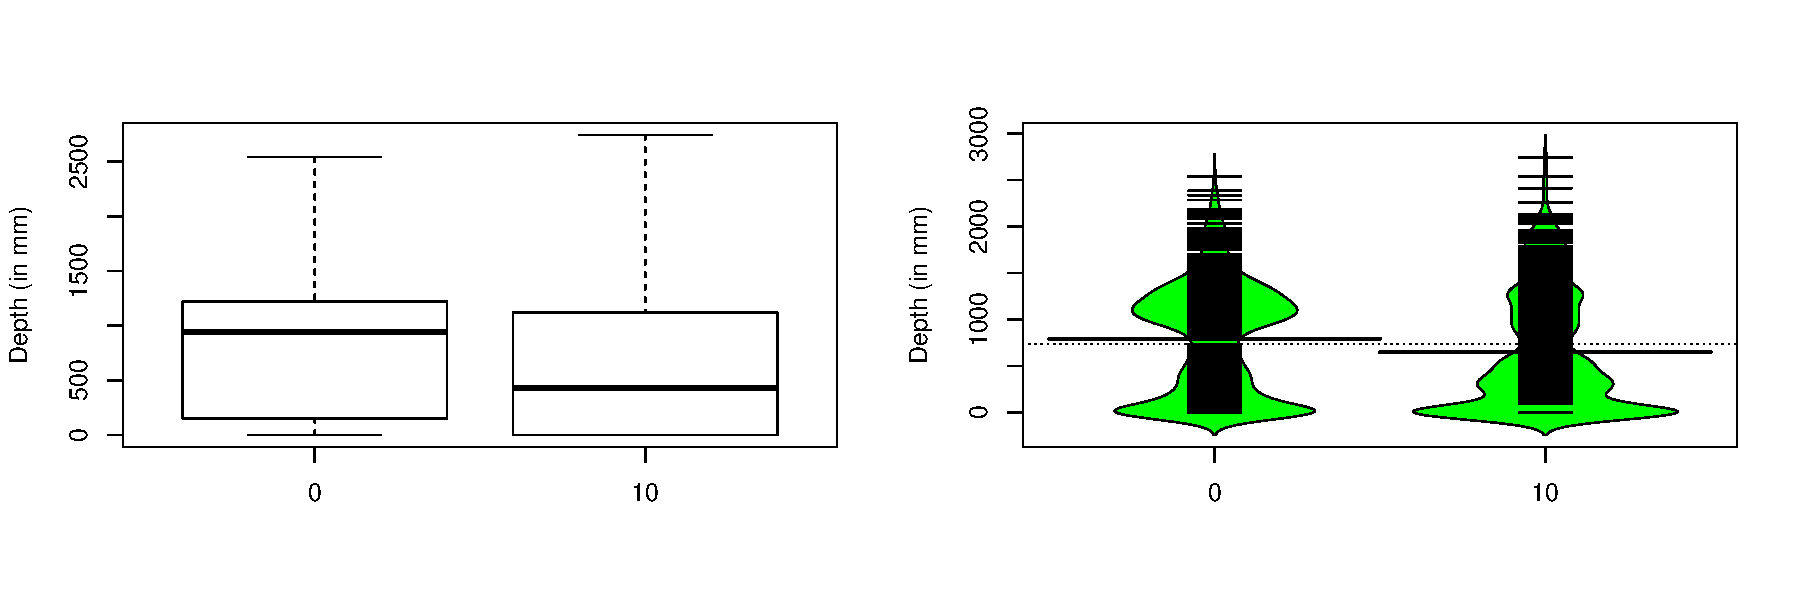
\includegraphics[width=\linewidth,height=0.3\linewidth]{figure/3-1} 

}



\end{knitrout}

\begin{exam}{Activity}

\begin{problem}
Does it appear from the summary measures or from the beanplots that there may be an association between forest cover and snow depth, on average? Explain.

\begin{solution}[2cm]
Yes, the mean snow depth for forested location appears smaller than the mean snow depth of unforested locations based on the beanplots and the sample means.
\end{solution}
\end{problem}

\subsection*{Hypotheses for the test}

\begin{problem*}
What is the null hypothesis of the test?

\begin{parts}
\item Using proper notation (making sure to define all parameters used):
\begin{solution}[2cm]
$H_0: \mu_{unf} = \mu_{for}$ where $\mu_{unf}$ is the true mean snow depth of unforested locations in the West Fork Basin and $\mu_{for}$ is the true mean snow depth of forested locations in the West Fork Basin.
\end{solution}
  \item In words:
  \begin{solution}[2cm]
There is no association between forest cover and snow depth in the West Fork Basin.
\end{solution}
  \item Write out the null model making sure to define all parameters used:
  \begin{solution}[2cm]
$y_{ij} = \mu + \varepsilon_{ij}$ where $\varepsilon_{ij} \sim{} N(0,\sigma^2)$ is the random error and $\mu$ is the true mean snow depth of any location in the West Fork Basin.
\end{solution}
\end{parts}
\end{problem*}


\begin{problem*}
What is the alternative hypothesis of the test?

\begin{parts}
\item Using proper notation (making sure to define all parameters used):
\begin{solution}[2cm]
$H_A: \mu_{unf} \neq \mu_{for}$ where $\mu_{unf}$ is the true mean snow depth of unforested locations in the West Fork Basin and $\mu_{for}$ is the true mean snow depth of forested locations in the West Fork Basin.
\end{solution}
  \item In words:
  \begin{solution}[2cm]
There is an association between forest cover and snow depth in the West Fork Basin.
\end{solution}
  \item Write out the null model making sure to define all parameters used:
  \begin{solution}[2cm]
$y_{ij} = \mu_j + \varepsilon_{ij}$ where $\varepsilon_{ij} \sim{} N(0,\sigma^2)$ is the random error and $\mu_j$ is the true mean snow depth for locations in the West Fork Basin that are forested ($j=1$) or locations that are unforested ($j=2$)
\end{solution}
\end{parts}
\end{problem*}

\subsection*{Assess the validity conditions}

\begin{problem}
{\bf Independence of observations:} The `observations' were the locations that snow depth was measured. The West Fork Basin was split into sampling areas to make the data collection process more feasible. The areas were selected to ensure all of the Basin could be reasonably accounted for. As such, the sampling areas themselves were not random (although they may be representative of the Basin itself). However, within each area a random location was chosen to obtain the snow depth measurements. As a result, there is weak evidence to suggest a clustering of observations or that the observations are related in any way.
\end{problem}
\begin{problem}
{\bf Equal variances in the groups:} We see from the beanplots above that the spreads, or variability, of the distributions of snow depth are similar for each group providing little evidence against this assumption.
\end{problem}
\begin{problem*}
  \begin{parts}
  \item {\bf Normal distributions of the observations in each group (parametric):} The distributions are not symmetric as the distribution of snow depth for the forested locations is right-skewed and the distribution of snow depth for the unforested locations is bimodal. There are really large sample sizes with 614 snow depth measurements at unforested locations and 403 snow depth measurements at forested locations. With these large sample sizes, due to the Central Limit Theorem, this assumption becomes less problematic.
  \item {\bf Similar distributions of the observations in each group (nonparametric):} The distributions are not similar as the distribution of snow depth for the forested locations is right-skewed and the distribution of snow depth for the unforested locations is bimodal (and left-skewed based on how the mean snow depth compares to the median snow depth).
  \end{parts}
\end{problem*} 


\subsection*{Find the value of the appropriate test statistic}

\begin{problem*}
Use {\tt t.test()} to calculate the test statistic. (This is the test statistic for both the parametric and nonparametric approaches.)

\begin{knitrout}\footnotesize
\definecolor{shadecolor}{rgb}{1, 1, 1}\color{fgcolor}\begin{kframe}
\begin{alltt}
\hlcom{# calculate the test statistic}
\hlstd{Tobs} \hlkwb{<-} \hlkwd{t.test}\hlstd{(depth} \hlopt{~} \hlstd{cover,} \hlkwc{data} \hlstd{= snow,} \hlkwc{var.equal} \hlstd{= T)}\hlopt{$}\hlstd{statistic}
\hlstd{Tobs}
\end{alltt}
\begin{verbatim}
##        t 
## 3.710287
\end{verbatim}
\end{kframe}
\end{knitrout}

\begin{parts}
\item What is the value of the test statistic and what type of statistic is it (t-statistic, z-statistic, F-statistic, etc.)?
\begin{solution}[1cm]
$t = 3.71$, it is a t-statistic
\end{solution}
  \item What was the order of subtraction in order to get the test statistic?
  \begin{solution}[1cm]
Unforested - Forested
\end{solution}
\end{parts}
\end{problem*}

\subsection*{Find the p-value}

\begin{problem*}
Use {\tt t.test()} to calculate the p-value using a parametric approach
\begin{knitrout}\footnotesize
\definecolor{shadecolor}{rgb}{1, 1, 1}\color{fgcolor}\begin{kframe}
\begin{alltt}
\hlcom{# parametric t test}
\hlkwd{t.test}\hlstd{(depth} \hlopt{~} \hlstd{cover,} \hlkwc{data} \hlstd{= snow,} \hlkwc{var.equal} \hlstd{= T,} \hlkwc{conf.level} \hlstd{=} \hlnum{0.95}\hlstd{)}
\end{alltt}
\begin{verbatim}
## 
## 	Two Sample t-test
## 
## data:  depth by cover
## t = 3.7103, df = 1015, p-value = 0.0002183
## alternative hypothesis: true difference in means is not equal to 0
## 95 percent confidence interval:
##   69.10668 224.26647
## sample estimates:
##  mean in group 0 mean in group 10 
##         793.5228         646.8362
\end{verbatim}
\end{kframe}
\end{knitrout}
\begin{parts}
  \item Under the null hypothesis, what is the sampling distribution of the test statisic?
  \begin{solution}[2cm]
Under the null hypothesis, the t-statistic follows a t-distribution with 1015 degrees of freedom. What this means is that if there were no association between forest cover and snow depth then a sample of size 1017 would yield a t-statistic value with probabilities determined by the t-distribution with 1015 degrees of freedom.
\end{solution}

\item What is the value of the p-value? Interpret this value in the context of the study.
\begin{solution}[2cm]
p-value=0.0002: This means that there approximately is a 0.02\% chance of observing a difference in mean snow depth as or more extreme then the difference oberved in the West Fork Basin, if there truly is no association between forest cover and snow depth.
\end{solution}
\end{parts}
\end{problem*}


\begin{problem*}
Use permutations to {\bf build} the null distribution (a nonparametric approach):
\begin{knitrout}\footnotesize
\definecolor{shadecolor}{rgb}{1, 1, 1}\color{fgcolor}\begin{kframe}
\begin{alltt}
\hlstd{B} \hlkwb{<-} \hlnum{2000}  \hlcom{## number of permutations we will perform}
\hlstd{Tstar} \hlkwb{<-} \hlkwd{matrix}\hlstd{(}\hlnum{NA}\hlstd{,} \hlkwc{nrow} \hlstd{= B)}  \hlcom{## empty slots for storage}
\hlkwd{set.seed}\hlstd{(}\hlnum{3}\hlstd{)}  \hlcom{## good practice when dealing with randomness}
\hlkwa{for} \hlstd{(b} \hlkwa{in} \hlnum{1}\hlopt{:}\hlstd{B) \{}
    \hlcom{## calculate the t statistic obtained from each shuffle}
    \hlstd{Tstar[b]} \hlkwb{<-} \hlkwd{t.test}\hlstd{(depth} \hlopt{~} \hlkwd{shuffle}\hlstd{(cover),} \hlkwc{data} \hlstd{= snow,} \hlkwc{var.equal} \hlstd{= T)}\hlopt{$}\hlstd{statistic}
\hlstd{\}}
\hlkwd{pdata}\hlstd{(}\hlkwd{abs}\hlstd{(Tstar),} \hlkwd{abs}\hlstd{(Tobs),} \hlkwc{lower.tail} \hlstd{= F)}  \hlcom{## obtain a p-value}
\end{alltt}
\begin{verbatim}
## t 
## 0
\end{verbatim}
\end{kframe}
\end{knitrout}
\begin{knitrout}\footnotesize
\definecolor{shadecolor}{rgb}{1, 1, 1}\color{fgcolor}

{\centering 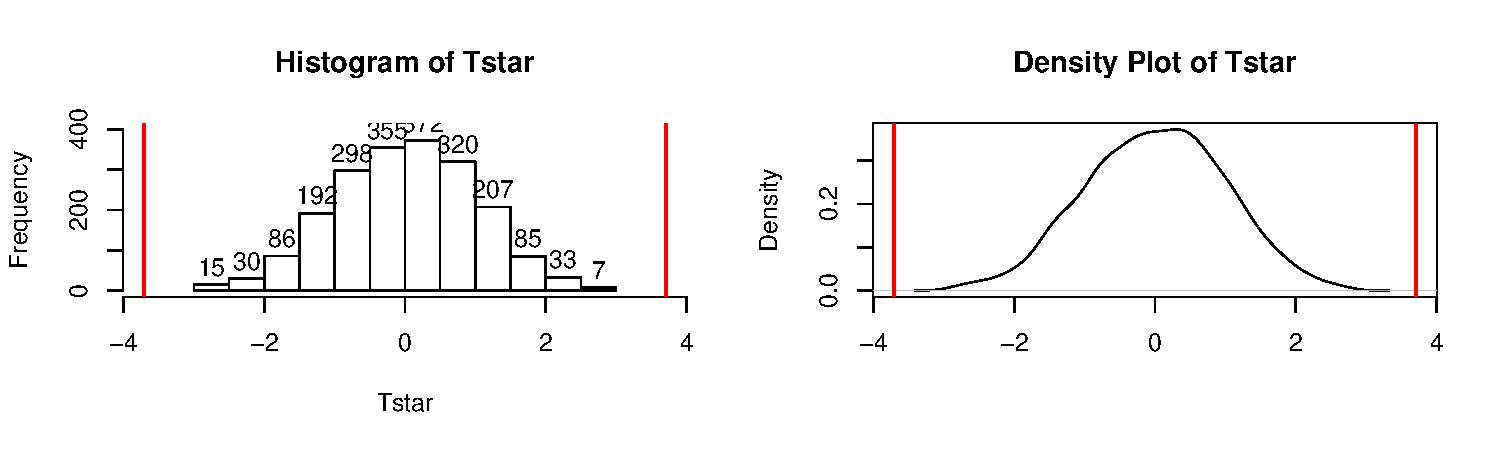
\includegraphics[width=\linewidth,height=0.3\linewidth]{figure/7-1} 

}



\end{knitrout}
\begin{parts}
  \item How many of the permutations resulted in a test statistic as or more extreme than the one observed in the original sample?
\begin{solution}[0.5cm]
0 or none
\end{solution}

\item What is the value of the p-value? ({\bf Note:} If your p-value$=0$ then you should say p-value $<0.001$.)
\begin{solution}[0.5cm]
The output says the p-value is 0, but we know that there exists at least one permutation with a t-statistic as or more extreme than our observed one (that is the one observed). Therefore the p-value $<0.001$.
\end{solution}

\item Compare the sampling distributions of the test statistic under the null hypothesis between non-parametric (permutations) and parametric ($t_{1015}$) using the following plot.
\begin{knitrout}\footnotesize
\definecolor{shadecolor}{rgb}{1, 1, 1}\color{fgcolor}

{\centering 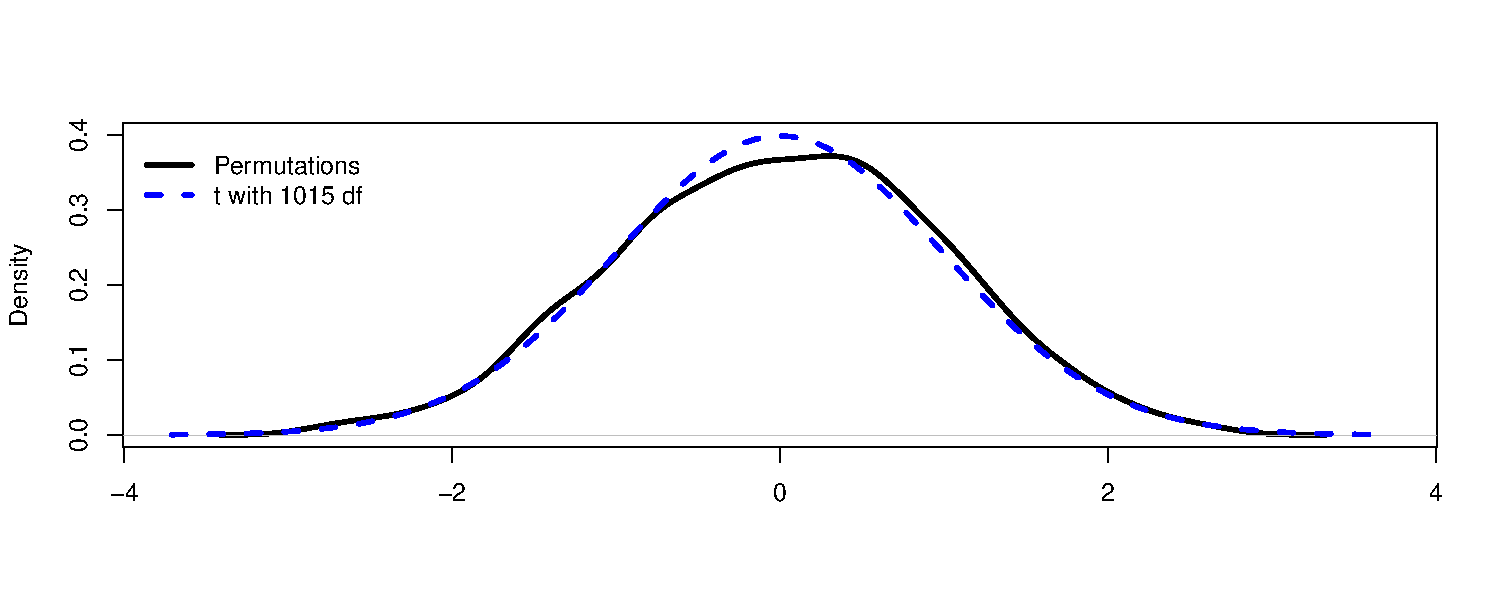
\includegraphics[width=0.5\linewidth,height=0.3\linewidth]{figure/8-1} 

}



\end{knitrout}
\begin{solution}[2cm]
The spreads and shapes are very similar. The p-value obtained should be roughly equal between the two methods.
\end{solution}
\end{parts}
\end{problem*}



\subsection*{Make a decision}
\begin{problem}
Make a decision for the test at the $\alpha=0.05$ significance level.
\begin{solution}[1cm]
At the 5\% significance level, we reject the null hypothesis.
\end{solution}
\end{problem}


\subsection*{Write a conclusion}
\begin{problem}
Write a conclusion specific to the problem, including scope of inference discussion.
\begin{solution}[2cm]
There is very strong evidence to support the claim that there is an association between forest cover and snow depth in the West Fork Basin. As the forest cover (forested or not) was not randomly assigned to locations we cannot infer a causal relationship between forest cover and snow depth. As the locations were randomly sampled from the areas in the West Fork Basin, we can infer this association holds for all areas in the West Fork Basin.
\end{solution}
\end{problem}



\pagebreak

\subsection*{Estimate the difference in means}
\begin{problem}
Calculate the point estimate for the difference in means, including the notations. Make sure to label it correctly (that includes the order of subtraction).

\begin{knitrout}\footnotesize
\definecolor{shadecolor}{rgb}{1, 1, 1}\color{fgcolor}\begin{kframe}
\begin{alltt}
\hlcom{## estimate the difference in means}
\hlstd{Tobs_d} \hlkwb{<-} \hlkwd{diffmean}\hlstd{(depth} \hlopt{~} \hlstd{cover,} \hlkwc{data} \hlstd{= snow)}
\hlstd{Tobs_d}
\end{alltt}
\end{kframe}
\end{knitrout}

\begin{solution}[1cm]
$\bar{x}_{unf} - \bar{for}_0 = -146.69$ mm
\end{solution}
\end{problem}


\begin{problem}
Report the 95\% confidence interval from problem 8. Was this CI obtained parametrically or nonparametrically?
\begin{solution}[2cm]
The parametrically obtained CI: (69.11, 224.27) \bf Note: \it The order of subtraction from \tt t.test() \it was unforested - forested, the \tt diffmean() \it function does the subtraction differently.
\end{solution}
\end{problem}


\begin{problem}
Now find the 95\% confidence interval using bootstrapping. Is this CI being obtained parametrically or nonparametrically?

\begin{knitrout}\footnotesize
\definecolor{shadecolor}{rgb}{1, 1, 1}\color{fgcolor}\begin{kframe}
\begin{alltt}
\hlcom{## bootstrap}
\hlstd{B} \hlkwb{<-} \hlnum{1000}  \hlcom{#we will resample 1000 times}
\hlkwd{set.seed}\hlstd{(}\hlnum{5}\hlstd{)}
\hlstd{Tboot} \hlkwb{<-} \hlkwd{matrix}\hlstd{(}\hlnum{NA}\hlstd{,} \hlkwc{nrow} \hlstd{= B)}  \hlcom{#empty slots for each statistic}
\hlkwa{for} \hlstd{(b} \hlkwa{in} \hlnum{1}\hlopt{:}\hlstd{B) \{}
    \hlcom{# different from the text but is more in line with 216 methods}
    \hlstd{Tboot[b]} \hlkwb{<-} \hlkwd{diffmean}\hlstd{(depth} \hlopt{~} \hlstd{cover,} \hlkwc{data} \hlstd{=} \hlkwd{resample}\hlstd{(snow,} \hlkwc{groups} \hlstd{= cover))}
\hlstd{\}}

\hlcom{## calculate the 95% CI}
\hlkwd{qdata}\hlstd{(Tboot,} \hlkwd{c}\hlstd{(}\hlnum{0.025}\hlstd{,} \hlnum{0.975}\hlstd{))}
\end{alltt}
\begin{verbatim}
##         quantile     p
## 2.5%  -228.37730 0.025
## 97.5%  -71.39043 0.975
\end{verbatim}
\end{kframe}
\end{knitrout}
\begin{solution}[1cm]
The nonparametrically obtained CI: (-228.38, -71.39) mm
\end{solution}
\end{problem}


\begin{problem}
Interpret the confidence interval from 14 in the context of the study.
\begin{solution}[2cm]
We are 95\% confident that the true mean snow depth of forested locations in the West Fork Basin is between 228.38 mm and 71.39 mm less than the true mean snow depth of unforested locations in the West Fork Basin.
\end{solution}
\end{problem}


\begin{problem}
Does your confidence interval from 14 match the decision for the test based on (9b)? Explain.
\begin{solution}[2cm]
Yes. We found that our confidence interval for the difference in true means did not contain 0, meaning value of 0 (the null hypothesized value) is not a plausible value the difference in true mean snow depths. If it is not a plausible value, then we should reject the null hypothesis, which is what we did in (9b).
\end{solution}
\end{problem}






\end{exam}

\end{document}
